\section{Design Space for In-Application Video Examples}
\label{sec:liveclips_designspace}
To help inform our decisions in developing LiveClips and explore how users might interact with such a system during their creative workflow, we outlined a design space for systems that present contextual video examples (\autoref{fig:liveclips_designspace}). This design space is informed by our formative findings as well as prior work on contextual assistance in software. The following three sections present the LiveClips system, which includes three alternative interfaces that explore three different points in this space. This section also highlights where RePlay and ReMap (Chapters \ref{chapter:replay}-\ref{chapter:remap}) fit in the design space as compared to LiveClips. Most notably, LiveClips differs from RePlay and ReMap in that it presents inspirational content rather than educational, and it presents short tool-focused clips rather than entire task-focused videos.

\begin{figure}[b!]
\centering
  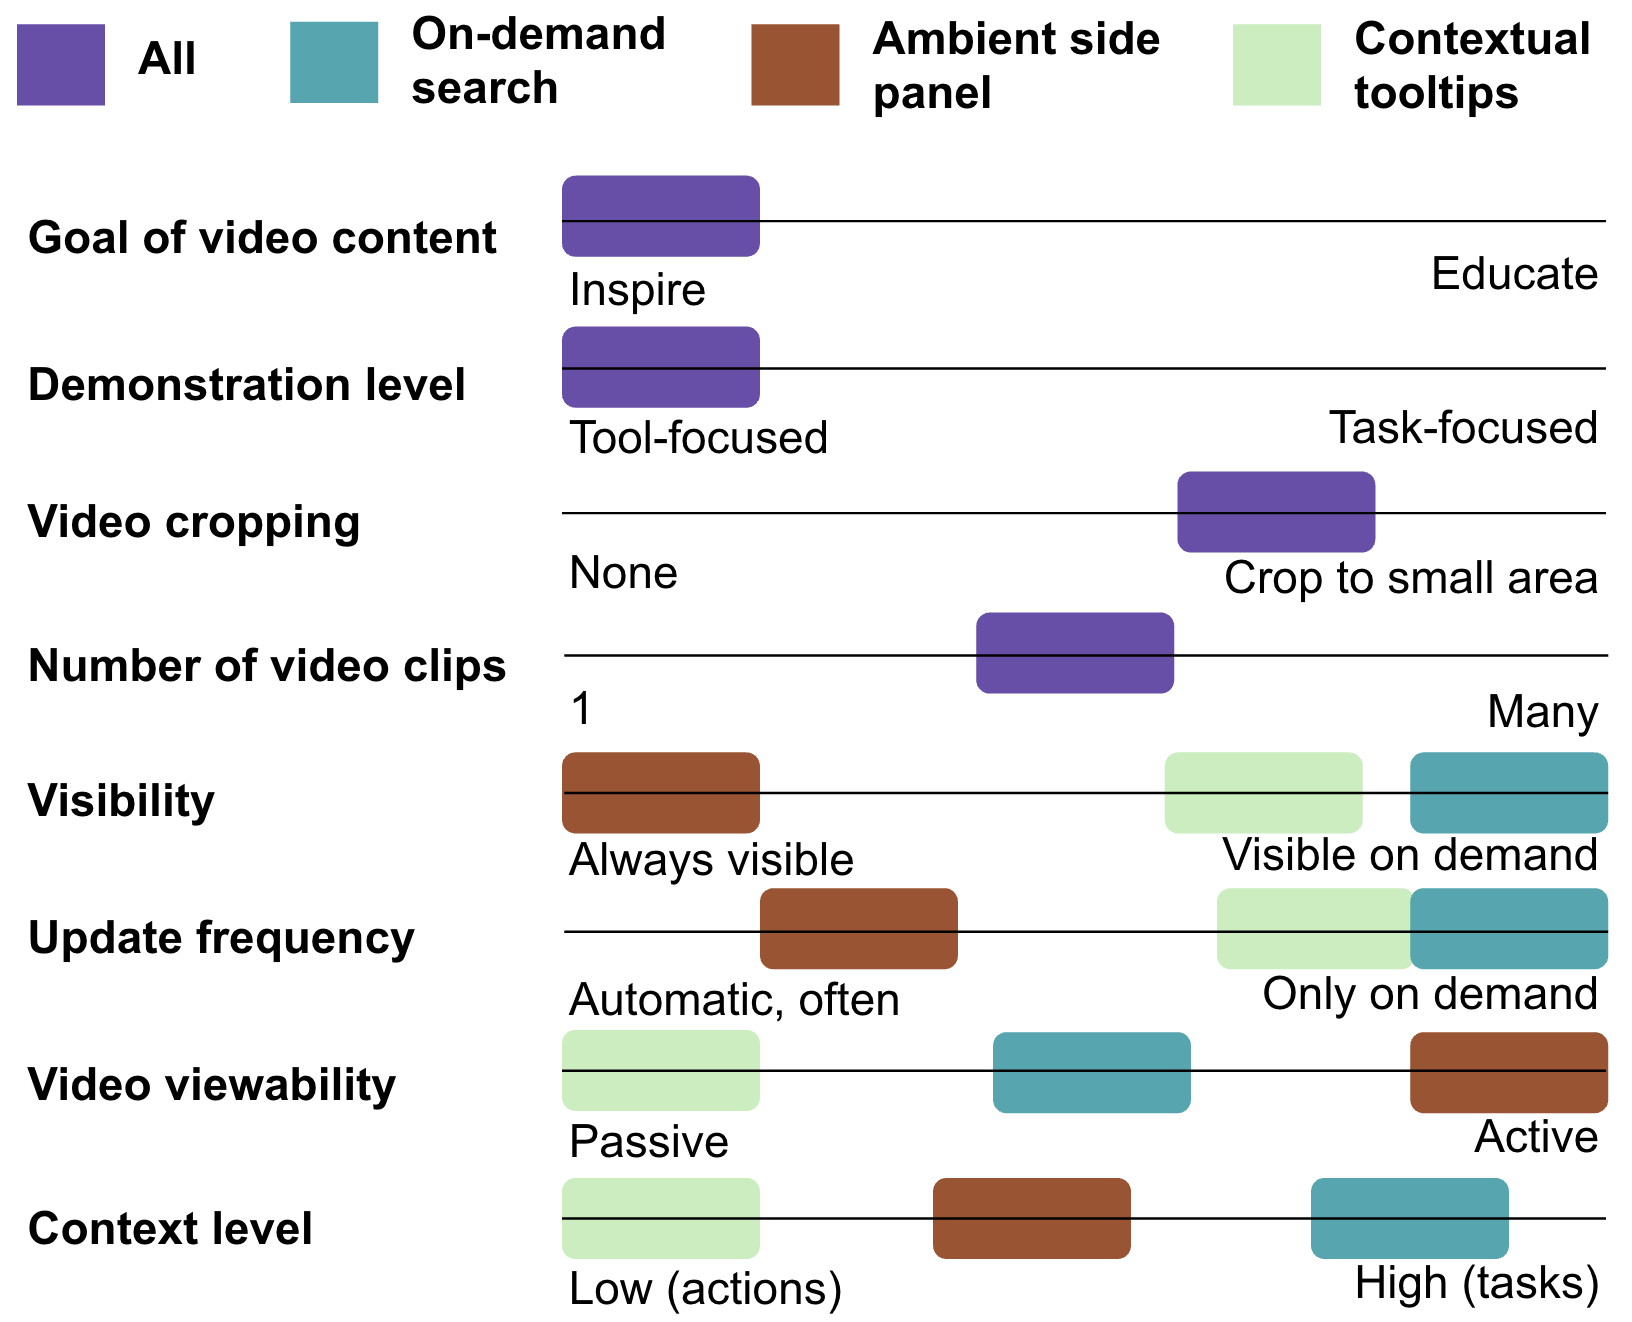
\includegraphics[width=\columnwidth]{liveclips/figures/designspace.png}
  \caption{The design space for in-application video examples, as well as where LiveClips and RePlay/ReMap fit along each axis. LiveClips' prototype interfaces vary along the bottom four axes. }~\label{fig:liveclips_designspace}
\end{figure}

\subsection{Goal of Video Content}
Most prior work regarding contextual videos, including RePlay and ReMap, has focused on content that aims to educate the user, such as tutorials \cite{Pongnumkul2011} and helpful tips \cite{Grossman2010a}. Inspired by the known benefits of examples for inspiration \cite{Kulkarni2014} and our survey findings suggesting that live streamed videos are used for inspiration, this work explores how contextual live streamed videos might inspire users. These videos also have educational value, but this work focuses on them as a source of inspiration.

\subsection{Demonstration Level}
Videos of software use can be tool-focused or task-focused. A tool-focused video demonstrates using a single tool, while a task-focused video shows an entire task from beginning to end.  Tool-focused videos are useful for quick contextual help that does not take away from the user's current work, for example reminding the user how a tool works \cite{Grossman2010a} or showing alternative uses for a tool.
Task-focused videos tend to be longer and are less useful in-the-moment, as they show a specific task that may or may not be relevant. Live streams tend to be task-focused, as they usually follow an artist through an entire task; this work focuses on extracting shorter, more generalizable tool-focused examples from task-focused live streams. RePlay and ReMap also extract relevant moments from within longer task-focused videos, but unlike LiveClips, they are meant for users who proactively seek help with a particular task, so they allow the user to browse the entire video and follow along with it.

%The likelihood that this task will be directly relevant to the user is low \cite{?}. 
%In this work, we focus on creating short tool-focused clips out of longer task-focused videos based on the assumption that shorter bite-sized clips are more useful as in-context recommendation, as they do not take the user away from their current work like a long task-focused clip would. 
%In addition, videos of artists using software often highlight alternative uses for tools that viewers may not have seen before, and so seeing a variety of ways a tool can be used may provide both inspirational and educational value. 

%Many of today's popular creative software applications support a wide variety of workflows. As a result, many of their tools can be used for multiple different purposes and in different contexts. Even expert software users may not be aware of all the different ways a tool can be used. Thus we expect that in addition to providing inspiration, tool-based clip recommendations may help increase users' awareness of the different ways tools can be used. By narrowing in on a focused aspect of a video, we also provide this content in a way that does not detract too much from the task at hand, unless the user wants to see more.

\subsection{Video Cropping}
In-application examples are constrained by space; if content takes up too much space it becomes obtrusive, for example by blocking the canvas where the user is currently working. Therefore, contextual videos must be displayed at a relatively small size. For videos that were created using full-screen video capture (as most live streams are), this can be problematic. Leaving a video un-cropped allows the user to see the full context of interaction but makes it difficult to discern any detail. Since RePlay and ReMap left videos un-cropped, they allowed users to open a single video in a larger window when seeing more detail was necessary. While this may have been practical for task-focused learning where users have other cues to indicate a video's relevance before selecting one (\textit{e.g.}, caption previews), LiveClips aims to show users many examples at once of tool use that may only take place in a small part of the screen. Prior work has explored how to best present video demonstration clips when they cannot be viewed in full screen, by cropping or enlarging sections in the video where mouse movement and canvas changes occur \cite{Chi2012}. Inspired by this, LiveClips crops videos to the area that shows the most visual change, in an effort to make examples focused and easy to browse.

\subsection{Number of Video Clips Shown}
Examples could be displayed one at a time, taking up the least amount of space but also providing less variety. Alternatively, displaying many videos gives users more options but potentially overwhelms them. Prior research on contextual videos recommends displaying multiple videos to demonstrate the range of uses for a tool and increase the likelihood that the user will find at least one useful \cite{Lafreniere2014, Matejka2011}. Similar to RePlay and ReMap (which displayed five videos at a time), our prototypes display four videos at a time in an effort to provide some variety without overwhelming the user or taking up too much space.

\subsection{Visibility}
Examples can be always visible while the user is working (like with RePlay and ReMap), or visible only on demand. Examples that are always visible are more likely to be seen but can be distracting, while examples that are not easily visible and shown only on request are more likely to be ignored or missed \cite{Rhodes1996}. Different users may have different preferences for how visible they want their examples to be, just as some viewers like to watch creative live streams while they work, while others may not. Our prototypes explore three variations along this axis.

\subsection{Update Frequency}
Recommended examples can update in response to an explicit user action (\textit{e.g.}, a query), an implicit user action (\textit{e.g.}, being idle for some time or opening a new document), or automatically at a regular time interval. Updating in response to explicit user actions was appropriate for RePlay and Remap, which are intended to be used when users have a specific question. But for a system like LiveClips that aims to elicit inspiration, the ideal approach is less clear. The trade-offs between these strategies have been widely explored in the literature, and it seems there is no globally optimal solution \cite{Rhodes1996, Chan2017, Siangliulue2015}. Automatic updates can be useful because they require zero effort from the user and can highlight an example in the moment \cite{Rhodes1996}, but they can also distract the user during periods of focused work \cite{Chan2017} or make the interface feel uncontrollable \cite{ODonovan2015}. Updates in response to an explicit request are less distracting and give the user more control over their attention but rely on the user to know when an update would be useful \cite{Rhodes1996, Siangliulue2015}. Update frequency is also tied to Visibility; recommendations that are only visible on-demand only update (visibly) when the user requests them. As with Visibility, the ideal solution may depend on the user's preferences; our prototypes explore three variations.

\subsection{Video Viewability}
When presenting non-static content such as videos in-app, the way in which the user interacts with and views the content may affect its usefulness. On the passive end, videos could play automatically when the content appears, which removes the need for the user to decide whether or not to watch a video but runs the risk of being distracting. On the other end, videos could be shown as a static thumbnail that only animates when the user intentionally interacts. Most prior work  \cite{Grossman2010a, Chi2012}, including RePlay and ReMap, has adopted the latter approach, however such work also suggests that in-context content should have a low threshold for engagement; the user shouldn't have to break too much from their task to interact with recommended content \cite{Grossman2010a}. LiveClips explores three variations along this axis.

\subsection{Context Level}
Examples can vary in how contextual they are to the user's behaviour. Low-level examples respond to the user's individual actions, such as the tools they use. High-level examples respond to the user's task or intent, which can be inferred from sequences of commands or by analyzing the document being edited. RePlay and ReMap use low-level context to augment queries, but the queries themselves can be either low- or high-level depending on the user. LiveClips mostly focuses on lower-level examples, but one of our three prototypes explores a potential way to measure task-level similarity between the user's actions and the examples clip's source video.